\documentclass[10pt]{article}

\usepackage[margin=0.72in]{geometry}
\usepackage{booktabs}
\usepackage{caption}
\usepackage{enumitem}
\usepackage{float}
\usepackage[T1]{fontenc}
\usepackage{graphicx}
\usepackage{hyperref}
\usepackage{microtype}
\usepackage{tabularx}
\usepackage{xcolor}

\hypersetup{
  colorlinks=true,
  linkcolor=blue!55!black,
  urlcolor=blue!55!black,
  citecolor=blue!55!black
}

\setlength{\parindent}{0pt}
\setlength{\parskip}{0.55em}
\setlength{\emergencystretch}{2em}
\setlist[itemize]{leftmargin=1.35em, itemsep=0.22em, topsep=0.25em}
\captionsetup{font=small, labelfont=bf}

\newcommand{\code}[1]{\texttt{#1}}
\newcommand{\splitkey}[1]{\texttt{#1}}

\title{\vspace{-1.2em}\textbf{AhmedML Dataset Splits}}
\author{}
\date{}

\begin{document}
\maketitle
\vspace{-2.0em}

Deterministic train/validation/test splits for the
\href{https://huggingface.co/datasets/neashton/ahmedml}{AhmedML} dataset
\cite{ahmedml_dataset}. The split manifest is stored at
\code{splits/manifest.json} as a flat JSON object with keys named
\code{\{split\_name\}\_\{train,val,test\}} and case IDs that match the
on-disk run directories.

AhmedML contains 500 geometric variations of the Ahmed car body. The public
force/moment table contains all 500 runs. This split package intentionally does
not store the large per-run STL or PNG assets. The committed lightweight
artifacts are the manifest, aggregate CSVs, derived Chamfer/image metrics, and
diagnostic figures. The geometry split is generated from STL-surface Chamfer
scores in \code{data/chamfer\_metrics.csv}. The image-wake split is generated
from \code{UxMean} Y-4 centreline and near-base X-slice PNG scores in
\code{data/image\_metrics.csv}. The geometry-parameter table contains 499 rows;
run 500 is absent from that file, so the generator mean-imputes its geometry
parameters only for the nested data-efficiency ordering and records this in
\code{data/parameter\_geometry\_metrics.csv}.

\section*{Splits at a glance}

\begin{tabularx}{\textwidth}{@{}l l r r r X@{}}
\toprule
Split & Type & Train & Val & Test & What it tests \\
\midrule
\splitkey{full} & In-dist & 400 & 50 & 50 & Noether-compatible seed-42 random baseline split \\
\splitkey{medium} & In-dist & 133 & 50 & 50 & Data efficiency, 1/3 of \splitkey{full} training data \\
\splitkey{scarce} & In-dist & 67 & 50 & 50 & Data efficiency, 1/6 of \splitkey{full} training data \\
\splitkey{super\_scarce} & In-dist & 11 & 50 & 50 & Extreme data efficiency, 1/36 of \splitkey{full} training data \\
\splitkey{geometry} & OOD & 350 & 50 & 100 & STL-shape extrapolation using the top 20\% local Chamfer-isolation score \\
\splitkey{high\_drag} & OOD & 350 & 50 & 100 & High-drag extrapolation using the top 20\% \code{cd} \\
\splitkey{low\_drag} & OOD & 350 & 50 & 100 & Low-drag extrapolation using the bottom 20\% \code{cd} \\
\splitkey{image\_wake} & OOD & 350 & 50 & 100 & Image-derived wake extrapolation using the top 20\% \code{UxMean} Y-4 plus near-base X-slice score \\
\bottomrule
\end{tabularx}

\textbf{Difficulty ladders:}
\begin{itemize}
  \item Data efficiency: \splitkey{full} < \splitkey{medium} < \splitkey{scarce} < \splitkey{super\_scarce}, with fixed validation/test sets.
  \item OOD regimes: \splitkey{geometry}, \splitkey{high\_drag}, \splitkey{low\_drag}, and \splitkey{image\_wake}.
\end{itemize}

\section*{Which split should I use?}

\begin{itemize}
  \item \textbf{Simple baseline or literature compatibility}: \splitkey{full}
  \item \textbf{Data efficiency study}: compare \splitkey{super\_scarce}, \splitkey{scarce}, \splitkey{medium}, and \splitkey{full}
  \item \textbf{Geometry extrapolation}: \splitkey{geometry}
  \item \textbf{Targeted coefficient extrapolation}: \splitkey{high\_drag} or \splitkey{low\_drag}
  \item \textbf{Image-derived wake extrapolation}: \splitkey{image\_wake}
\end{itemize}

\section*{Using the committed splits}

For standard benchmark use, consume the committed manifest at
\code{splits/manifest.json}; no regeneration is required. The manifest is the
source of truth for all split membership and contains one train, validation,
and test key for each split listed above.

\begin{verbatim}
import json
from pathlib import Path

manifest = json.loads(Path("splits/manifest.json").read_text())

train_ids = manifest["geometry_train"]
val_ids = manifest["geometry_val"]
test_ids = manifest["geometry_test"]
\end{verbatim}

Change the \code{geometry} prefix to \code{full}, \code{medium},
\code{scarce}, \code{super\_scarce}, \code{high\_drag}, \code{low\_drag}, or
\code{image\_wake} to select a different split. Each value is a sorted list of
\code{run\_N} directory names that match the dataset case folders.

\section*{Design principles}

\begin{itemize}
  \item \textbf{Validation is always in-distribution with train.} For OOD splits, validation is drawn from the training-side population, not from the held-out extreme test region.
  \item \textbf{Keep the public baseline stable.} \splitkey{full} matches Noether's AhmedML seed-42 split: 400 train, 50 validation, and 50 test.
  \item \textbf{Use the source data for each regime.} Drag-regime splits use \code{force\_mom\_all.csv}; geometry-regime splits use externally downloaded STL files and \code{data/chamfer\_metrics.csv}; image-regime splits use externally downloaded \code{UxMean} PNG files and \code{data/image\_metrics.csv}.
  \item \textbf{Nested data-efficiency subsets.} \splitkey{super\_scarce\_train} is a strict subset of \splitkey{scarce\_train}, \splitkey{scarce\_train} is a strict subset of \splitkey{medium\_train}, and \splitkey{medium\_train} is a strict subset of \splitkey{full\_train}.
  \item \textbf{Test set integrity.} Test cases should not be used for hyperparameter tuning, model selection, normalization fitting, or visual inspection-driven iteration.
\end{itemize}

\section*{Split details}

\subsection*{\splitkey{full}}

The default public split is a seeded random split over all 500 run IDs, not a
physics-stratified split. It constructs \code{torch.randperm(500)} with seed
42, shifts the IDs to \code{1..500}, then assigns the first 400 IDs to train,
the next 50 to validation, and the final 50 to test. The case IDs are sorted
before being stored in the manifest. These IDs match the public
\href{https://github.com/Emmi-AI/noether/blob/main/src/noether/data/datasets/cfd/caeml/ahmedml/split.py}{AhmedMLDefaultSplitIDs}
implementation in Noether \cite{noether_split}.

\subsection*{\splitkey{medium}, \splitkey{scarce}, and \splitkey{super\_scarce}}

Same validation/test as \splitkey{full}, but the training set is a nested
force- and geometry-diverse subset of \splitkey{full\_train}: 133 cases for
\splitkey{medium}, 67 cases for \splitkey{scarce}, and 11 cases for
\splitkey{super\_scarce}. The subset order is a greedy max-min selection in
standardized force/geometry feature space using \code{cd}, \code{cl}, and all
available geometry parameters.

\subsection*{\splitkey{geometry}}

The geometry split is an STL-surface OOD split. Each \code{run\_N/ahmed\_N.stl}
is sampled with 4096 deterministic area-weighted surface points. The sampled
point clouds are compared using symmetric Chamfer RMS distance after scaling by
the global median STL bounding-box diagonal. The geometry score is the mean
Chamfer distance to the 10 nearest neighboring runs:

\begin{verbatim}
geometry_score_i = mean_10_nearest_neighbors(chamfer_distance_i)
\end{verbatim}

The top 20\% of runs by this local-isolation score form the OOD test set.
Validation is sampled from the remaining training-side pool:

\begin{verbatim}
geometry_test  = top_20_percent_i(geometry_score_i)
geometry_pool  = all_runs - geometry_test
geometry_val   = deterministic_random_sample(geometry_pool, round(0.125 * |geometry_pool|))
geometry_train = geometry_pool - geometry_val
\end{verbatim}

In the current metrics, the most locally isolated STL cases include
\splitkey{run\_52}, \splitkey{run\_153}, \splitkey{run\_244},
\splitkey{run\_480}, \splitkey{run\_410}, \splitkey{run\_96},
\splitkey{run\_431}, and \splitkey{run\_91}. Figure~\ref{fig:diagnostics}
shows the geometry split against the Chamfer score used to define the holdout.
Figure~\ref{fig:geometry_examples} shows a low-score and high-score geometry
example, with both STLs projected in the same coordinate frame.

\begin{figure}[H]
  \centering
  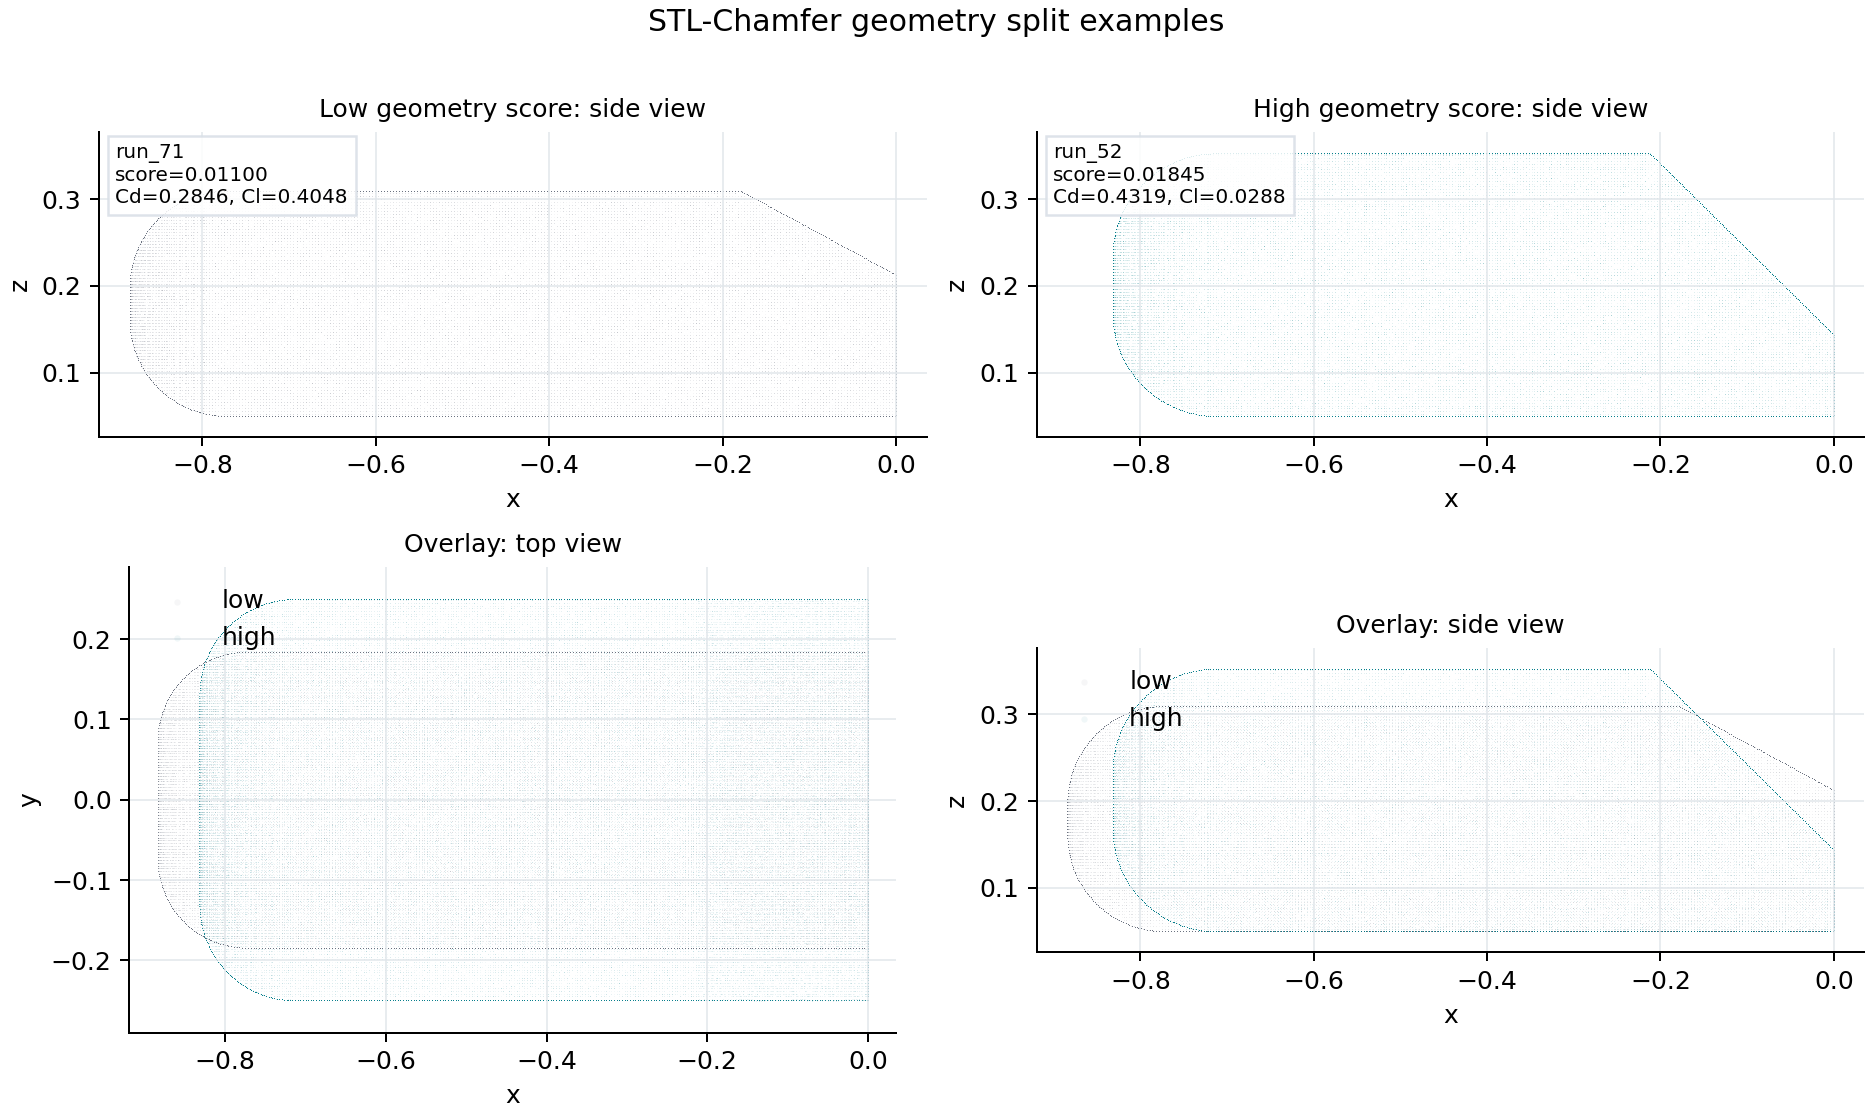
\includegraphics[width=0.96\textwidth]{geometry_score_examples.png}
  \caption{Geometry-score examples for \splitkey{geometry}. The low-score case is \splitkey{run\_71} with Chamfer score 0.010996, \code{Cd}=0.2846, and \code{Cl}=0.4048. The high-score case is \splitkey{run\_52} with Chamfer score 0.018450, \code{Cd}=0.4319, and \code{Cl}=0.0288. The lower panels overlay the low-score and high-score STL vertex projections in a common coordinate frame.}
  \label{fig:geometry_examples}
\end{figure}

\subsection*{\splitkey{high\_drag} and \splitkey{low\_drag}}

Both splits sort all 500 cases by drag coefficient \code{cd}.
\splitkey{high\_drag} holds out the top 20\% by \code{cd};
\splitkey{low\_drag} holds out the bottom 20\% by \code{cd}. In both cases,
train/validation are sampled from the complementary 80\% so validation remains
in-distribution with training. Figure~\ref{fig:diagnostics} shows these
holdouts across run IDs.

In the current CSV, the highest-drag runs include \splitkey{run\_362},
\splitkey{run\_205}, \splitkey{run\_284}, \splitkey{run\_280}, and
\splitkey{run\_315}. The lowest-drag runs include \splitkey{run\_390},
\splitkey{run\_238}, \splitkey{run\_122}, \splitkey{run\_117}, and
\splitkey{run\_10}.

\subsection*{\splitkey{image\_wake}}

The image-wake split is computed from downloaded \code{UxMean} PNGs under an
external asset directory with \code{run\_N/images/UxMean} subfolders. Each run contributes the \code{Y-4}
centreline/near-centreline side image plus three near-base cross-plane images:
\code{X-14}, \code{X-15}, and \code{X-16}. For each image, the script scores
the lower flow region using a reproducible color-intensity measure, then
combines the \code{Y-4} score with the mean near-base X score. The top 20\% of
runs by this image score form the OOD test set, and validation is sampled from
the complementary training-side pool. Figure~\ref{fig:diagnostics} shows both
the score used to define \splitkey{image\_wake} and the same split colored on
drag coefficient.

In the current metrics, the highest image-wake scores include
\splitkey{run\_280}, \splitkey{run\_205}, \splitkey{run\_284},
\splitkey{run\_309}, \splitkey{run\_315}, \splitkey{run\_362},
\splitkey{run\_171}, and \splitkey{run\_295}.
Figure~\ref{fig:wake_examples} compares the lowest and highest image-wake
score cases using the \code{Y-4} centreline image and a nearer-base \code{X-14}
image from the same PNG source used by the score.

\begin{figure}[H]
  \centering
  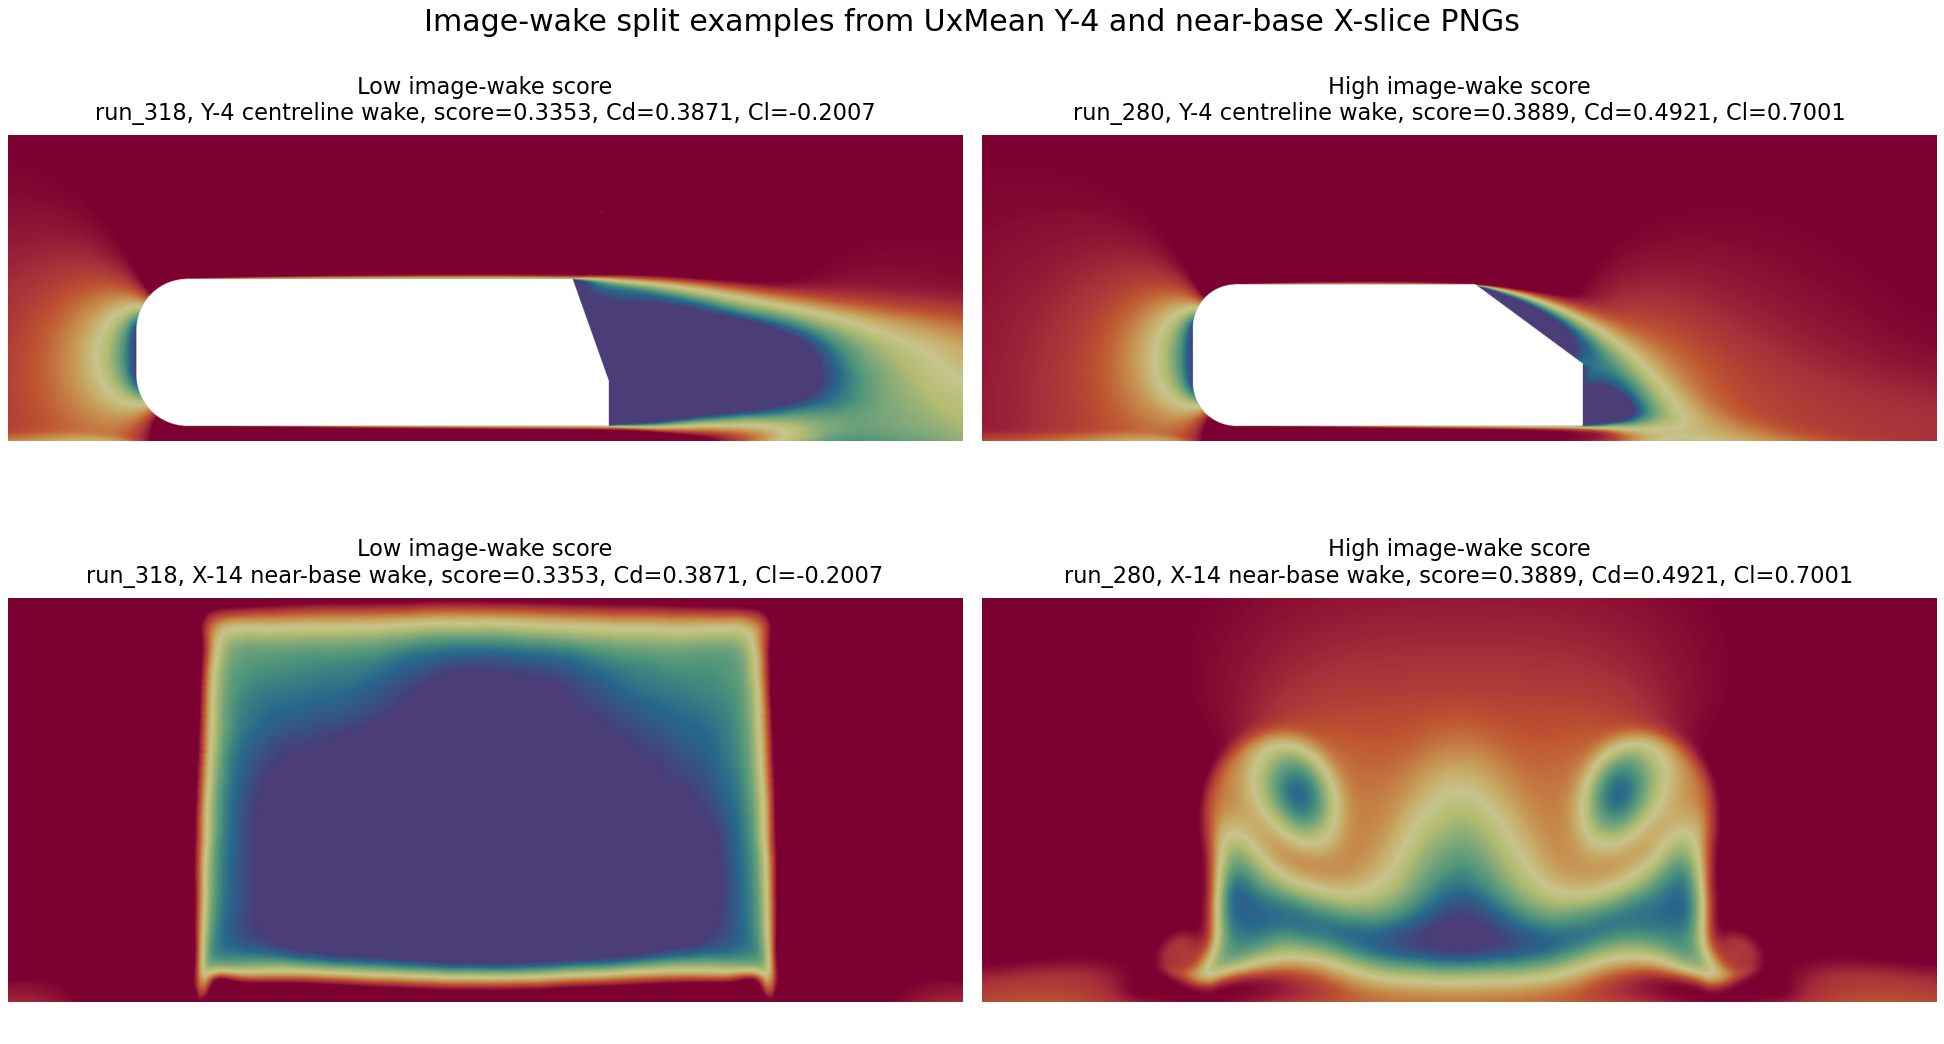
\includegraphics[width=0.96\textwidth]{wake_score_examples.png}
  \caption{Image-wake examples for \splitkey{image\_wake}. The low-score case is \splitkey{run\_318} with image score 0.3353, \code{Cd}=0.3871, and \code{Cl}=-0.2007. The high-score case is \splitkey{run\_280} with image score 0.3889, \code{Cd}=0.4921, and \code{Cl}=0.7001. The top row shows \code{Y-4}, which captures the centreline wake, and the bottom row shows the nearer-base \code{X-14} slice.}
  \label{fig:wake_examples}
\end{figure}

\begin{figure}[H]
  \centering
  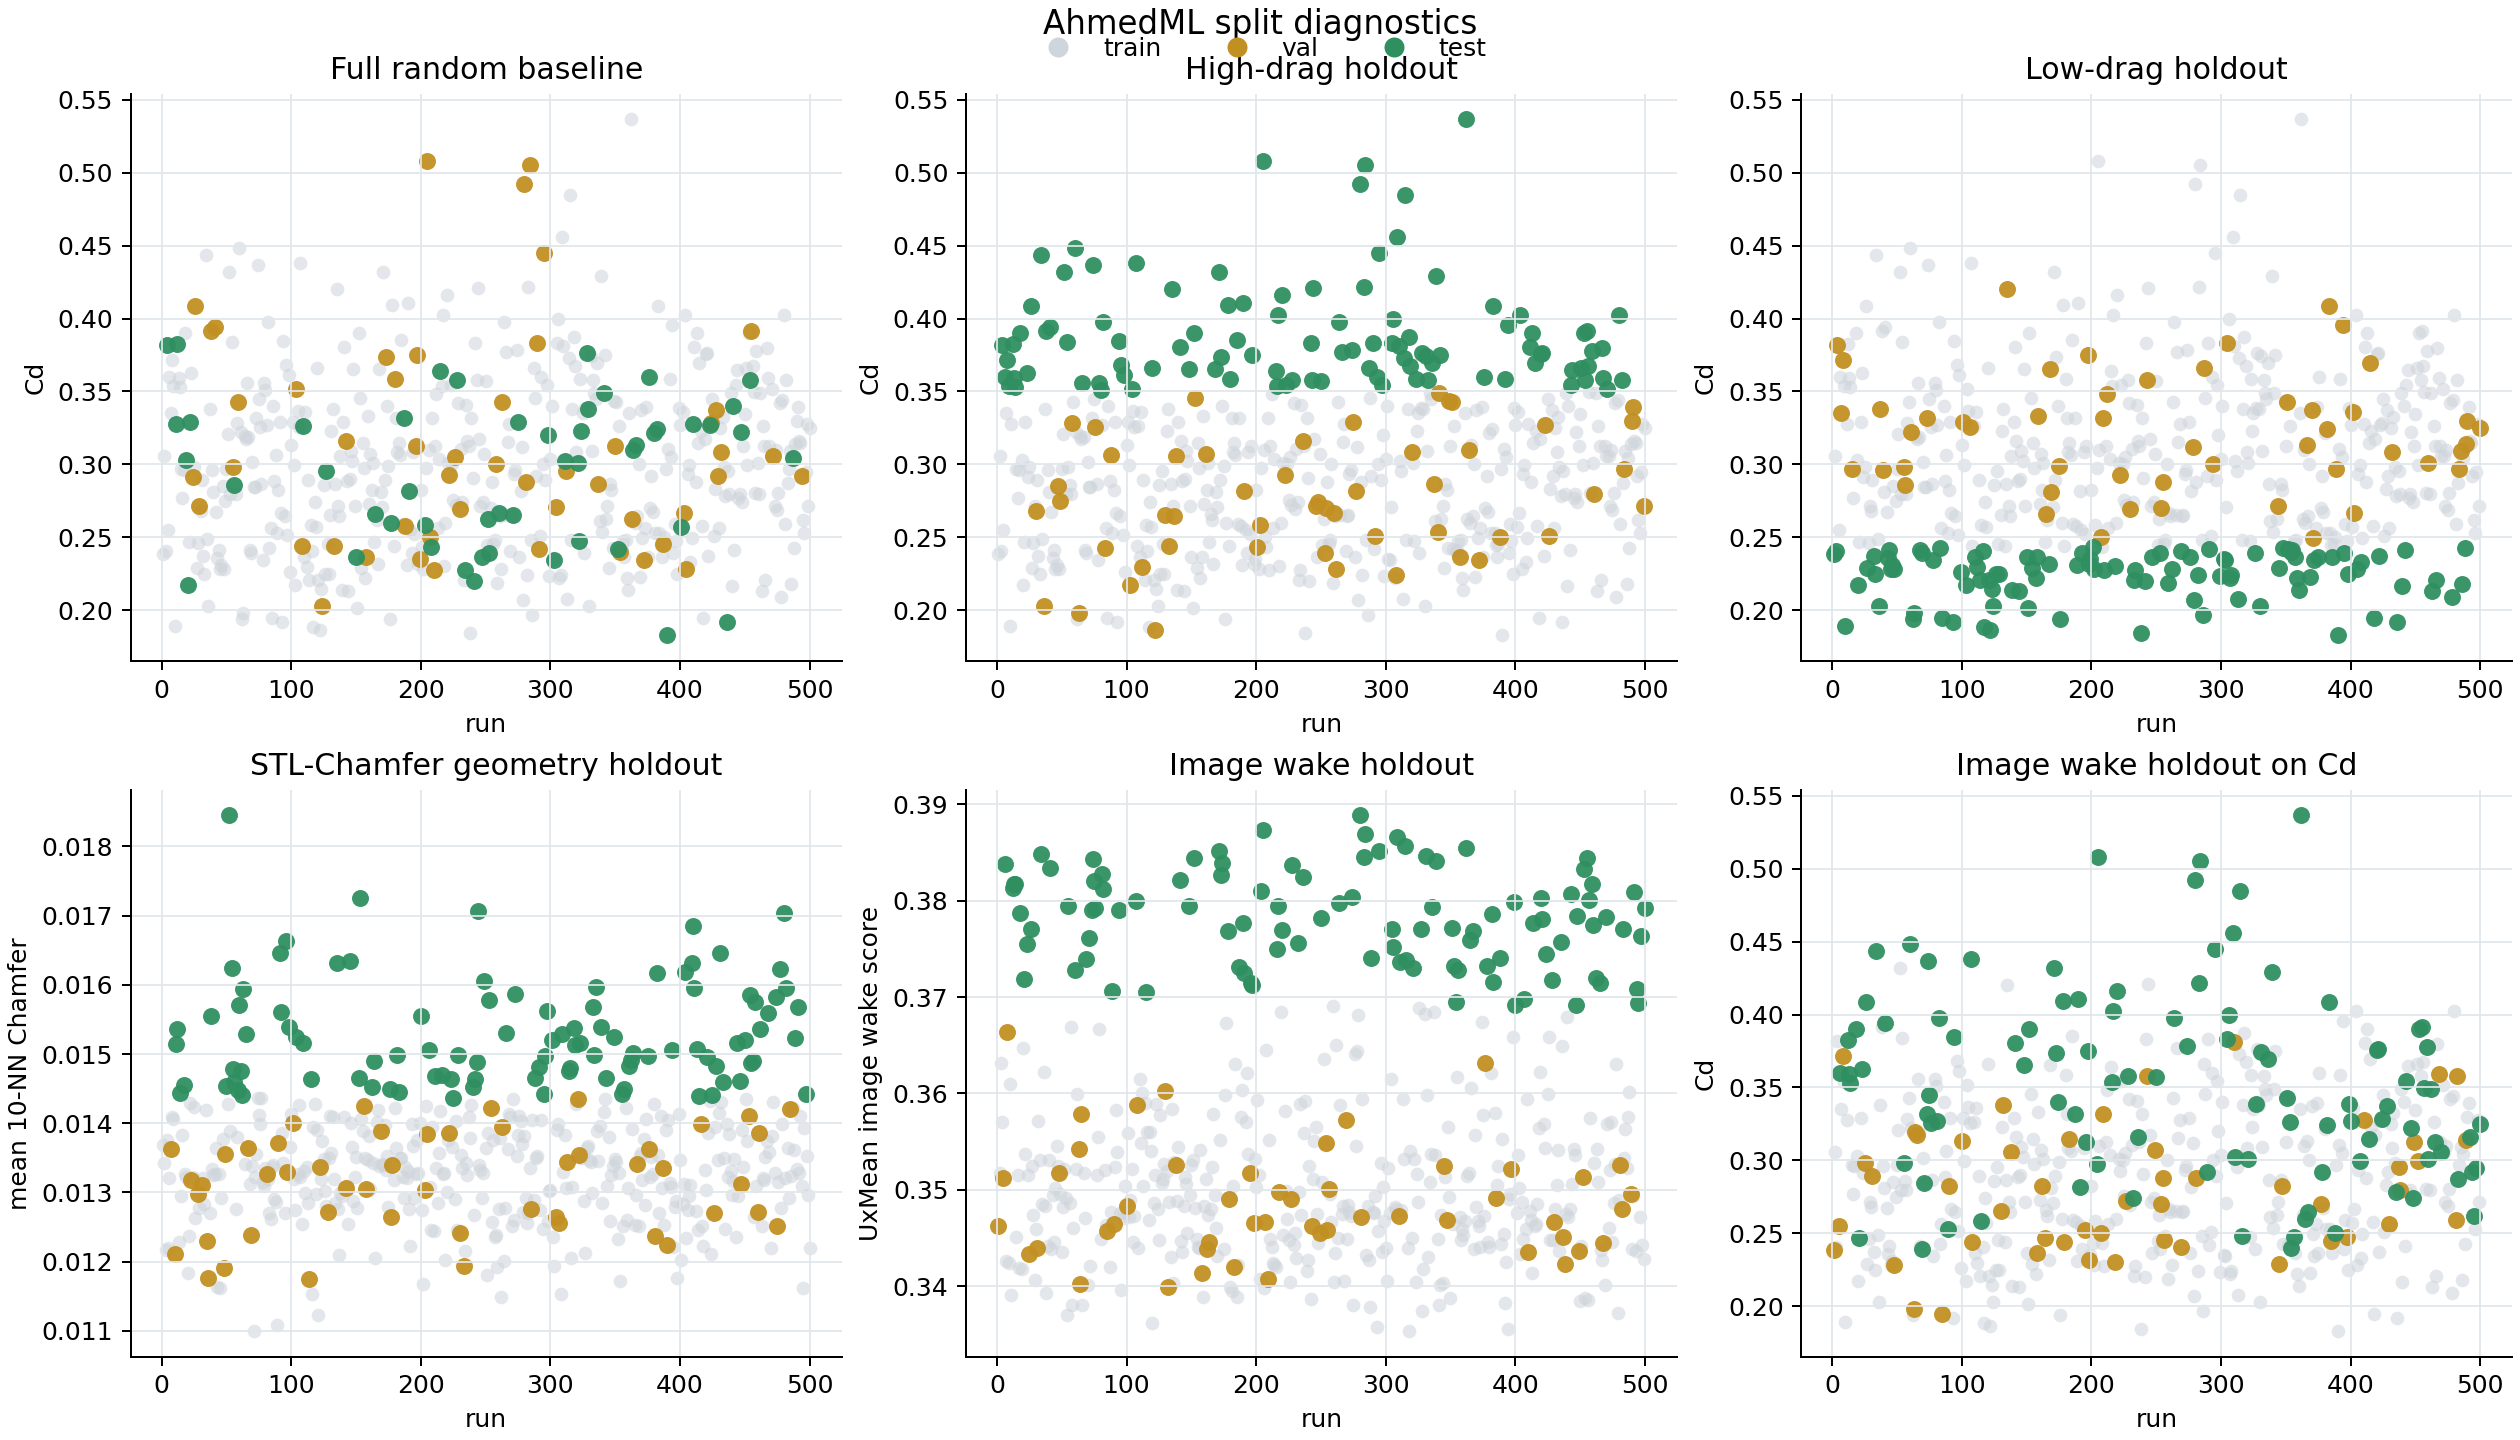
\includegraphics[width=0.96\textwidth]{split_diagnostics.png}
  \caption{AhmedML split diagnostics. The panels show the full random baseline, high-drag holdout, low-drag holdout, STL-Chamfer geometry holdout, image-wake holdout, and image-wake split colored on \code{Cd}. The x-axis is run ID, and points are colored by each split's train, validation, and test partitions.}
  \label{fig:diagnostics}
\end{figure}

\section*{Repeatability and transparency}

The committed manifest is intended for normal use. The commands below are for
auditing the split construction, recreating the figures, or refreshing the
artifacts after changing the source data.

From a clean split-package checkout, download \code{force\_mom\_all.csv},
\code{geo\_parameters\_all.csv}, STLs, and the \code{UxMean} PNGs needed for
the image-wake split into a directory outside this repository, then regenerate
the metrics, manifest, and diagnostic plot:

\begin{verbatim}
ASSET_ROOT=../ahmedml_hf_assets

python3 scripts/download_hf_inputs.py --output-dir "$ASSET_ROOT" \
  --include-stls --include-wake-images --workers 6
python3 scripts/compute_chamfer_splits.py --data-root "$ASSET_ROOT" \
  --output-dir /tmp/ahmedml_chamfer_4096 --samples 4096 \
  --workers 16 --sample-workers 2 --runs all \
  --base-manifest splits/manifest.json
cp /tmp/ahmedml_chamfer_4096/chamfer_metrics.csv data/chamfer_metrics.csv
python3 scripts/compute_image_metrics.py --data-root "$ASSET_ROOT" \
  --output data/image_metrics.csv
AHMEDML_DATA_ROOT="$ASSET_ROOT" python3 scripts/generate_splits.py
python3 scripts/visualize_splits.py
python3 scripts/create_example_figures.py --asset-root "$ASSET_ROOT"
\end{verbatim}

Full report regeneration then uses:

\begin{verbatim}
latexmk -pdf -cd docs/README.tex
\end{verbatim}

For an existing dataset checkout, set \code{AHMEDML\_DATA\_ROOT} to the
directory containing \code{force\_mom\_all.csv} and
\code{geo\_parameters\_all.csv}. Set \code{AHMEDML\_ASSET\_ROOT}, or pass
\code{--asset-root}, to the directory containing the \code{run\_*/} STL and
PNG assets. The repository's own \code{data/} directory should remain limited
to small CSV files.

The committed source artifacts were generated against:

\begin{verbatim}
data/force_mom_all.csv
data/geo_parameters_all.csv
<asset-root>/run_*/ahmed_*.stl
<asset-root>/run_*/images/UxMean/*.png
data/chamfer_metrics.csv
data/image_metrics.csv
data/parameter_geometry_metrics.csv
docs/geometry_score_examples.png
docs/wake_score_examples.png
splits/manifest.json
\end{verbatim}

\section*{Manifest format}

\begin{verbatim}
{
    "full_train": ["run_1", "run_2", "..."],
    "full_val": ["run_24", "..."],
    "full_test": ["run_4", "..."],
    "scarce_train": ["run_10", "..."]
}
\end{verbatim}

Case IDs match on-disk directory names and are sorted numerically by run number.

{\small
\begin{thebibliography}{9}
\bibitem{ahmedml_dataset}
AhmedML dataset. \url{https://huggingface.co/datasets/neashton/ahmedml}.

\bibitem{ahmedml_paper}
AhmedML paper. \url{https://arxiv.org/abs/2407.20801}.

\bibitem{noether_split}
Noether AhmedML split. \url{https://github.com/Emmi-AI/noether/blob/main/src/noether/data/datasets/cfd/caeml/ahmedml/split.py}.
\end{thebibliography}
}

\end{document}
